%!TEX root=../book.tex

\chapter{Simple Linear Regression}

\section{Overview of Simple Linear Regression}

\subsection{Uses of Simple Linear Regression}
In the last chapter we touched briefly on the idea of using the value of one variable to predict the value of another. Where correlation is used to describe the magnitude of the relationship between two variables, a tool called \textbf{simple linear regression} takes that relationship and uses it to predict the values of Variable B, given some arbitrary value of Variable A. In this context, however, we refer to the \(x\) variable as our \textbf{explanatory variable} or our \textbf{regressor} and to the \(y\) variable as the \textbf{response variable}.

So, knowing that we use regression as a predictive tool, what \textit{is} it, exactly? Well, thankfully, it's a pretty straightforward thing that we can define as:

\begin{equation}
y = \beta_0 + \beta_1\cdot x
\label{eqn:regression01}
\end{equation}

So before we explain this equation, we need you to reach way back into those murky memories of your eighth grade math class when you were talking about the equation of a line. Remember that whole ``slope-intercept form'' lecture? Well, in case you don't, the equation of a line looks something like:
\begin{equation*}
y=m\cdot x+b
\end{equation*}
where $m$ is the slope and $b$ is the intercept. Sound familiar?

Alright, now let's compare those two equations. Aside from using different variable names, they're identical to one another. All regression boils down to is drawing lines to connect a bunch of points on the page. And here you thought it was going to be scary!

Although regression is actually a bit more than drawing a line to connect the dots, the basic idea behind it is that for two variables there exists an equation with two basic constants---a slope and an intercept---that allows us to predict the value of $Y$ if we already know $X$.

But, although we know that equation exists, how do we figure it out? To do that we'll turn to something called \textbf{least squares estimators}.

\subsection{Least Squares Fitting}

If you think back to Equation \ref{eqn:regression01}, our two coefficients were $\beta_0$ and $\beta_1$. Those refer to the population coefficients: that is, if we were able to measure every single instance of $X$ and $Y$ in all of the universe, those would be the coefficients that we could derive from the population. In most cases, however, that isn't possible and so we use least squares estimates of $\beta_0$ and $\beta_1$ which we refer to as $\hat{\beta}_0$ and $\hat{\beta}_0$ (pronounced ``beta-null hat'' and ``beta-one hat'').

We can visualize this process in Figure \ref{fig:regression01}. Here, we see a number of data points as white circles. There is also a solid black line that represents a possible line of best fit. However, are the predicted data points (solid black circles) as close to the observed data as possible? Looking at the red dashed line between our predictions and observations, it looks like we could do a better job reducing that difference.

\begin{figure}[h]
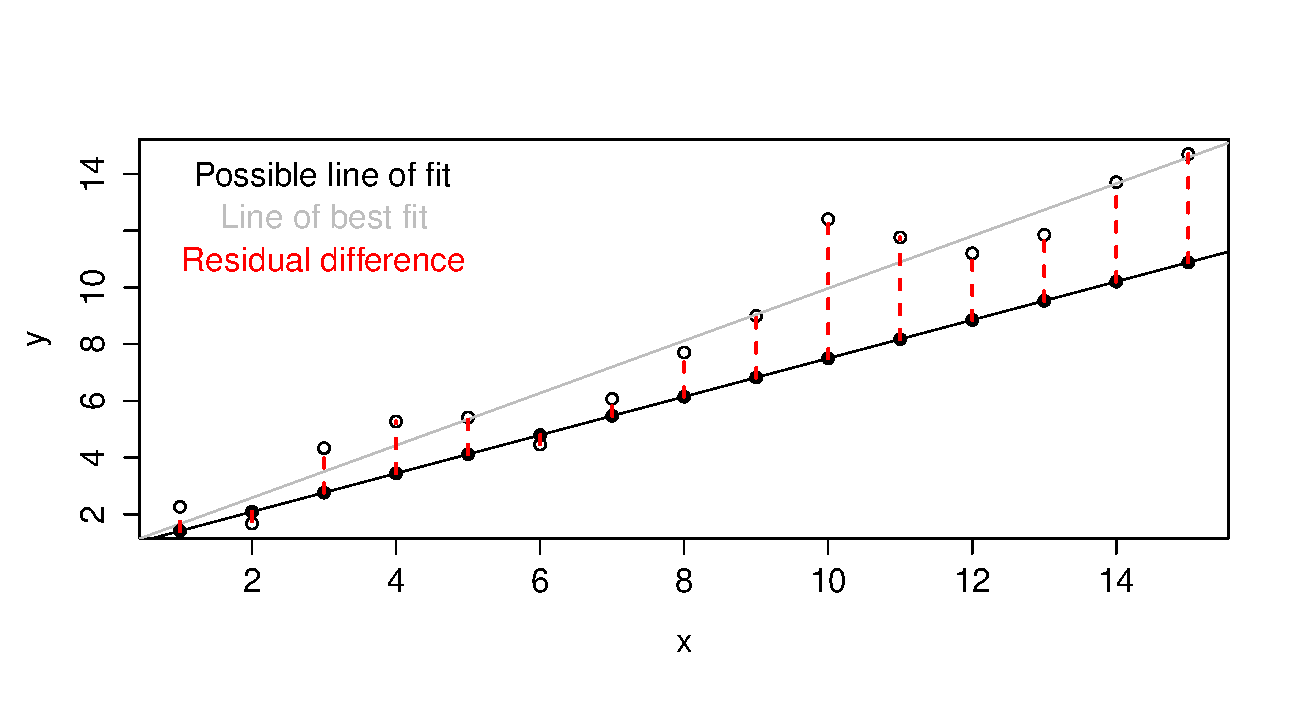
\includegraphics[width=35pc]{regression01}
\caption{Data with a least-squares line of best fit (grey), one potential line of best fit (black), and the residual difference between the predicted and observed values (red). Lease squares fitting seeks to minimize the overall distance between every observed value and predicted value, resulting in a single line of best fit.}
\label{fig:regression01}
\end{figure}

Minimizing that difference between our predicted and observed values is exactly what least squares estimation seeks to do. In fact, we can see the least squares line of best fit as the light grey line in Figure \ref{fig:regression01}. The residual difference in this line is mathematically as small as it possibly can be.

How we actually do this involves a bit of calculus so we aren't going to go into too much detail here. However, from that calculus we can derive these two estimates of our coefficients:
\begin{eqnarray*}
\hat{\beta}_1 &=& \frac{\sum_{i=1}^n\left(X_i-\bar{X}\right)\left(Y_i-\bar{Y}\right)}{\sum_{i=1}^n\left(X_i-\bar{X}\right)^2}\\
\hat{\beta}_0 &=& \bar{Y}-\hat{\beta}_1\cdot \bar{X}
\end{eqnarray*}

Thankfully, these aren't equations that you're liable to ever have to understand or use (unless you just really want to): least squares fitting is automated by every modern statistical package. Even your TI-84 calculator is happy to do it for you. The point, rather, is that given a set of data, there are these mathematical tools that we can use to attempt to model the relationship between our variables, even though this is mostly a behind-the-scenes operation.

\subsection{Coefficient of Determination}


\subsection{Residuals}


\section{Cautions and Considerations}


\subsection{Basic Assumptions}

page 182

\subsection{Outliers and Influential Points}


\section{Case Study: [STUDY]}


\section{Exercises}


\section{Additional resources}